\section{Related Work on Pruning}
Pruning is the most widely studied form of model compression, and it has been applied to Transformers in a variety of ways. The related work discussion is organized along two coupled axes: the topology of the induced sparsity pattern and the optimization signal used to identify removable units. This framing keeps the deployment question explicit from the outset, because similar nominal compression ratios may correspond to different execution regimes, different preprocessing costs, and different forms of realized speedup.

The section is organized as follows. We first establish the problem setting and the taxonomy used to classify methods. We then survey saliency-based, gradient-based, second-order, and proxy- and search-based approaches in turn, and close with a cross-method empirical comparison.

\subsection{Problem Setting and Taxonomy}

\newcommand{\methoddetail}[1]{%
    \par\medskip
    \noindent{\bfseries #1}\par
    \smallskip\noindent
}

Building on the formal framework introduced in Chapter~\ref{chap:neural_network_pruning}, the related-work discussion is organized along two coupled axes: the topology of the induced sparsity pattern and the optimization signal used to identify removable units. Before surveying individual methods, we establish the classification scheme that makes cross-method comparisons coherent.

\subsubsection{Taxonomy of Transformer Pruning Methods}

The three sparsity topologies (unstructured, semi-structured $N\!:\!M$, and structured) were introduced formally in Section~\ref{sec:pruning_structures} (see Figure~\ref{fig:structures}). From a deployment standpoint, they differ in whether pruning yields compressed storage alone, sparse-kernel acceleration, or native dense-shape acceleration after model surgery.

The taxonomy adopted here follows four coupled axes. The \emph{removable unit} determines whether the method acts on scalar weights, local N:M groups, or executable structures such as attention heads, FFN channels, and layers \cite{Michel2019,kurtic2022optimal}. The \emph{optimization signal} ranges from magnitude and activation statistics to differentiable mask learning, first-order Taylor criteria, second-order curvature surrogates, or search-based proxy objectives \cite{sun2023simple,xia2022structured,ma2023llmpruner,frantar2023sparsegpt,zhao2024pruning,kwon2022fast}. The \emph{recovery stage} distinguishes direct post-training pruning from methods requiring LoRA recovery, gradual fine-tuning, or distillation. The \emph{deployment objective} determines whether the reported benefit is compressed storage, sparse-kernel acceleration, dense-shape acceleration, or measured speedup \cite{kurtic2023ziplm,evopress2024,darwinlm2025}.

Each family corresponds to a different deployment objective. Unstructured methods such as Wanda and SparseGPT primarily optimize weight-level saliency \cite{sun2023simple,frantar2023sparsegpt}. Semi-structured methods such as MRP incorporate local coupling constraints matching N:M execution primitives \cite{zhao2024pruning}. Structured methods span differentiable mask-learning (CoFi), dependency-aware gradient methods (LLM-Pruner), Fisher-based post-training frameworks, and runtime-aware second-order methods (ZipLM) \cite{xia2022structured,ma2023llmpruner,kwon2022fast,kurtic2023ziplm}. Search-based methods such as EvoPress and DarwinLM treat pruning as configuration optimization under explicit budget or hardware constraints \cite{evopress2024,darwinlm2025}. Figure~\ref{fig:pruning_taxonomy} and Table~\ref{tab:pruning_taxonomy} summarize this organization.

\begin{figure}[htbp]
	\centering
	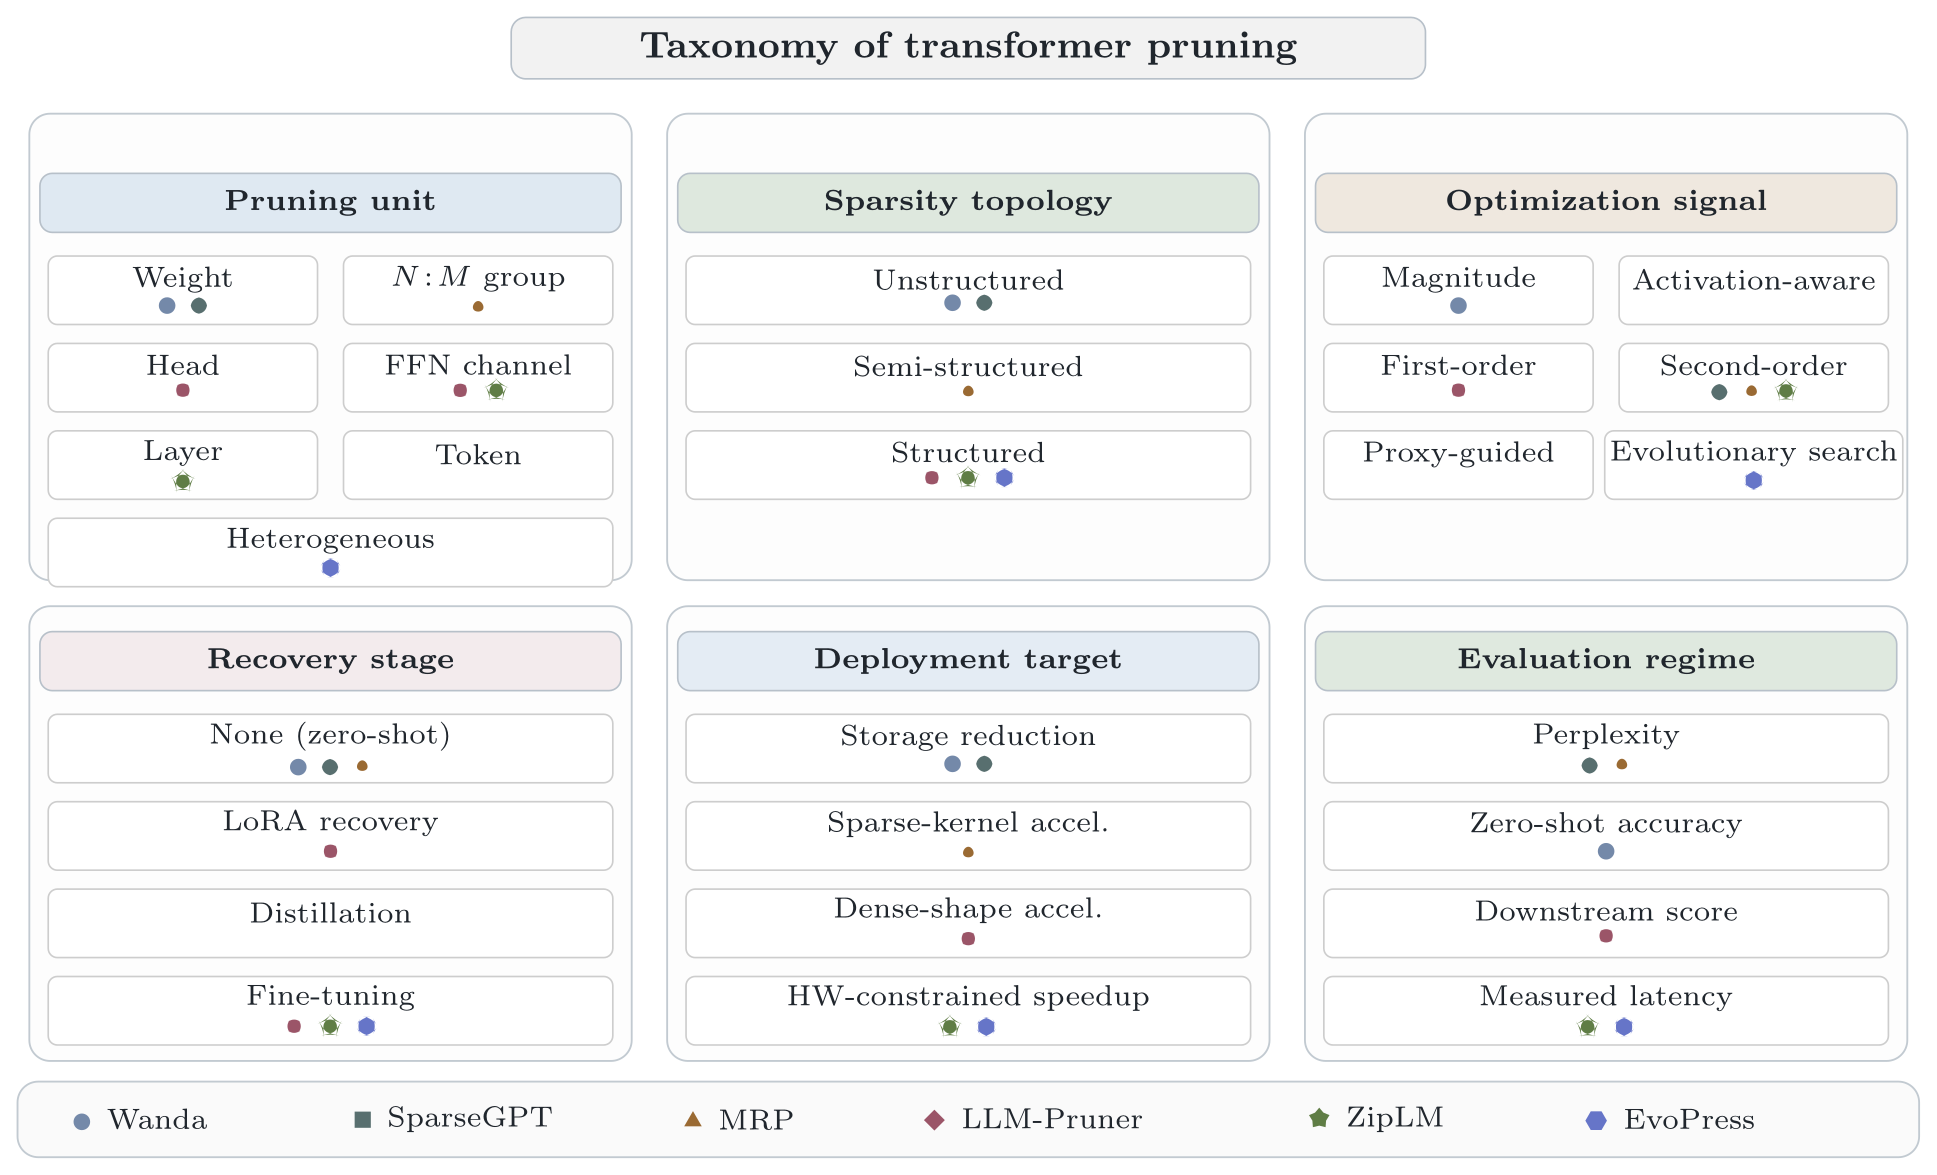
\includegraphics[width=0.96\textwidth]{figures/compression/transformer_pruning_taxonomy.png}
	\caption{Taxonomy of the pruning methods considered in this chapter. The classification crosses the pruning unit, sparsity topology, optimization signal, recovery stage, deployment objective, and evaluation regime.}
	\label{fig:pruning_taxonomy}
\end{figure}

\begin{table}[htbp]
	\centering
	\caption{Taxonomy used to organize the pruning methods discussed in this chapter}
	\label{tab:pruning_taxonomy}
	\begin{tabularx}{\textwidth}{l >{\raggedright\arraybackslash}X >{\raggedright\arraybackslash}X >{\raggedright\arraybackslash}X >{\raggedright\arraybackslash}X >{\raggedright\arraybackslash}X}
		\toprule
		\textbf{Method} & \textbf{Unit} & \textbf{Topology} & \textbf{Signal} & \textbf{Recovery} & \textbf{Primary deployment claim} \\
		\midrule
		Wanda & Weight & Unstructured & Activation-aware saliency & None & Zero-shot retention under storage-oriented sparsity \\
		CoFi & Layers / heads / FFN / hidden dimensions & Structured & Learned hard-concrete masks with $L_0$ control and distillation & Full task-specific pruning and fine-tuning & Dense-shape acceleration through jointly pruned Transformer structure \\
		LLM-Pruner & Heads / channels / blocks & Structured & First-order Taylor with dependency groups & LoRA recovery & Structural compression with dense-shape execution \\
		SparseGPT & Weight & Unstructured & Single-weight second-order compensation & None & High-sparsity pruning with local reconstruction \\
		MRP & N:M group & Semi-structured & Joint second-order compensation & None & Hardware-aligned N:M sparsity for sparse-kernel execution \\
		Fast post-training pruning & Heads / FFN filters & Structured & Fisher-based constrained mask optimization & None beyond mask tuning & FLOPs- or latency-constrained structured pruning without retraining \\
		ZipLM & Heads / FFN dimensions & Structured & Second-order structured saliency with runtime-constrained search & Gradual fine-tuning and distillation & Measured speedup under device-specific constraints \\
		EvoPress / DarwinLM & Layer-wise compression levels & Heterogeneous structured & Proxy-guided or evolutionary search & Search-time evaluation or proxy training & Pareto optimization under global budget and hardware constraints \\
		\bottomrule
	\end{tabularx}
\end{table}

The remainder of the section follows this taxonomy. Saliency-based methods provide low-overhead baselines. Gradient-based structured methods replace scalar saliency with group-aware masking over executable units. Second-order methods introduce curvature-aware reconstruction at weight level, structural level, and runtime-aware settings. Proxy- and search-based methods operate over configuration spaces rather than applying a single closed-form ranking rule.

\subsection{Saliency-Based Methods}

Saliency-based methods rely on zeroth-order saliency or activation statistics rather than explicit gradients, curvature surrogates, or population-based search. Their main advantages are low calibration budgets, limited preprocessing overhead, and simple implementation. Two representatives are examined here: plain magnitude pruning, which serves as the universal baseline, and Wanda, which extends magnitude ranking with activation-channel information.

\subsubsection{Magnitude and Activation-Aware Baselines}

This subsection covers two methods: plain weight-magnitude pruning, which forms the universal zero-cost baseline, and Wanda, which extends it with a single activation-channel factor derived from a small calibration set.

\paragraph{Weight-Magnitude Pruning.}
Magnitude pruning uses absolute weight values as the saliency proxy. Formally, the importance score assigned to weight $W_{i,j}$ at row $i$ and column $j$ is defined as:
\begin{equation}
	\mathcal{S}^{\mathrm{mag}}_{i,j} = |W_{i,j}|.
\end{equation}
Its core assumption is that small weights contribute less to the output and can be removed with limited degradation. The method requires no gradient-based recovery and remains the simplest baseline against which more sophisticated algorithms are evaluated.

\paragraph{Wanda (Weights $\times$ Activations).}
Wanda \cite{sun2023simple} refines this baseline by incorporating activation information from a small calibration set. Rather than relying on weight magnitude alone, it multiplies each weight by the $\ell_2$ norm of its input activation channel, giving the joint saliency score:
\begin{equation}
	\mathcal{S}^{\mathrm{wanda}}_{i,j} = |W_{i,j}| \cdot \|x_j\|_2,
\end{equation}
where $x_j$ is the $j$-th input activation channel and $\|x_j\|_2$ is its RMS norm estimated over $N$ calibration samples. The key insight is that importance is jointly encoded in weight magnitude and the energy of the coupled input channel.

\methoddetail{Algorithm Overview}
Wanda processes each layer independently: it collects input activations on a small calibration set (typically 128 samples), computes per-weight saliency scores as the product of weight magnitude and activation norm, then prunes the lowest-scoring weights for each output neuron until the target sparsity $p$ is reached. No weight update or recovery step is applied. Magnitude pruning is a pure linear scan $O(|W|)$ with no calibration; Wanda adds only an activation-collection pass, keeping the overall cost near-linear.

The two methods above represent the lightweight end of the pruning spectrum. The following section moves to methods that bring gradient information into the scoring process to enable structured, executable compression.

\subsection{Gradient-Based Methods}

These methods retain structured pruning objectives over heads, channels, or blocks, but replace simple magnitude heuristics with gradient-informed saliency criteria defined over executable groups. Two methods are discussed: LLM-Pruner, which uses dependency-aware Taylor scoring and LoRA-based recovery, and CoFi, which frames the entire pruning process as a differentiable joint mask-learning problem.

\subsubsection{Gradient-Based Dependency for Structured Units}

Structured pruning replaces individual-weight saliency with group-level importance. The natural units in Transformers are multi-head attention heads, FFN channels, and entire layers. A pruning decision must respect architectural dependencies propagated through residual pathways and projection matrices.

\paragraph{Minimally-Removable Units.}
Removing one attention head deletes its parallel path and the associated slices in $W_Q$, $W_K$, $W_V$, and $W_O$ \cite{Michel2019}. Pruning intermediate FFN neurons removes coordinated rows and columns in the two-layer MLP block \cite{kurtic2022optimal}. Layer dropping maximizes parameter removal per decision but carries a higher risk of representational collapse \cite{kim2021learned}.

\paragraph{LLM-Pruner: Dependency Groups, Taylor Scoring, and LoRA Recovery.}
LLM-Pruner \cite{ma2023llmpruner} first discovers \emph{dependency groups} so that every removed unit corresponds to a consistent structural change. In the paper's LLaMA setting, two granularities are used: \emph{block groups} covering coupled head/FFN structures, and \emph{channel groups} for dimension-style pruning across projection layers.

\methoddetail{Dependency Graph and Minimally-Removable Units}
Groups are identified by a dependency graph over neurons. To formalize which neurons must be pruned together, LLM-Pruner defines two propagation rules based on in-degree and out-degree. For neurons $N_i$ and $N_j$ with input set $\mathrm{In}(N)$ and output set $\mathrm{Out}(N)$, these rules determine when removing $N_i$ forces the removal of $N_j$, and vice versa:
\begin{align}
	N_j \in \mathrm{Out}(N_i) \wedge \deg^{-}(N_j)=1 &\implies N_j \text{ depends on } N_i, \label{eq:dep1}\\
	N_i \in \mathrm{In}(N_j) \wedge \deg^{+}(N_i)=1 &\implies N_i \text{ depends on } N_j. \label{eq:dep2}
\end{align}
The transitive closure defines one group $\mathcal{G}=\{W_i\}_{i=1}^M$; all weights in that group are pruned together.

\methoddetail{Taylor Scoring}
Once groups are identified, LLM-Pruner scores them with Taylor approximations of the loss increase on a small calibration set $\mathcal{D}$. To estimate how much removing a group would increase the task loss without running a full fine-tuning pass, the vector-wise importance of structure tensor $W_i$ is approximated as:
\begin{equation}
	I_{W_i}
	\approx
	\left|
	\frac{\partial \mathcal{L}^{\top}(\mathcal{D})}{\partial W_i}W_i
	-\frac{1}{2}W_i^{\top}HW_i
	\right|,
	\label{eq:taylor-vector}
\end{equation}
where $H$ is the local Hessian. Unlike classical second-order pruning, the first-order gradient is retained because calibration data are only a proxy for pretraining data. The element-wise variant replaces the diagonal Hessian term with a Fisher-diagonal approximation. Group importance is aggregated from individual tensor scores using sum, product, max, or last-only operators; groups with the smallest aggregate score are pruned first.

\methoddetail{Recovery Stage}
After pruning, LLM-Pruner applies LoRA adapters \cite{hu2021lora} to all linear modules. The low-rank update $\Delta W = PQ$ (rank $r=8$) is optimized with AdamW for two epochs over roughly 50K Alpaca-style samples. Because the factors can be merged back into $W$, the final model carries no adapter overhead at inference time. Recovery takes approximately 2.5 hours on a single RTX 4090. The scoring stage requires only 10 short calibration sequences for forward/backward passes, keeping the preprocessing cost practical.

\methoddetail{Algorithm Overview}
The pipeline proceeds in three stages. First, the Transformer computation graph is traversed to collect dependency groups following Equations~\eqref{eq:dep1} and \eqref{eq:dep2}. Second, Taylor scores are computed for each group on the calibration set and groups are ranked; the lowest-scoring groups are pruned until the target ratio $p$ is reached. Third, LoRA adapters are inserted into all linear modules, optimized on the recovery corpus, and merged back into the surviving weights.

\paragraph{CoFi: Joint Coarse- and Fine-Grained Structured Pruning.}
CoFi \cite{xia2022structured} treats structured pruning as differentiable mask learning over several coupled architectural units. To make every architectural granularity jointly controllable, CoFi augments the standard Transformer forward pass with binary gate variables at multiple levels. In each Transformer layer, explicit masks are introduced for attention blocks and FFN blocks so that the gated forward computations become:
\begin{align}
	\mathrm{MHA}(X) &= z_{\mathrm{MHA}} \sum_{i=1}^{N_h} z_{\mathrm{head}}^{(i)} \,\mathrm{Att}\!\left(W_Q^{(i)},W_K^{(i)},W_V^{(i)},W_O^{(i)},X\right), \\
	\mathrm{FFN}(X) &= z_{\mathrm{FFN}}\, \mathrm{gelu}(XW_U)\,\mathrm{diag}(z_{\mathrm{int}})\,W_D,
\end{align}
supplemented by a shared hidden-dimension mask $z_{\mathrm{hidn}}$. At high sparsity, explicit coarse masks allow the optimizer to remove complete MHA or FFN blocks directly.

\methoddetail{Hard-Concrete Mask Learning}
Each mask variable is optimized through the hard-concrete relaxation for $L_0$ regularization. The expected sparsity is controlled by a Lagrangian constraint, and to simultaneously enforce the sparsity budget and maintain task performance through teacher supervision, the full training objective is defined as:
\begin{equation}
	\mathcal{L}_{\mathrm{prune}}
	=
	\mathcal{L}_{\mathrm{task}}
	+
	\mathcal{L}_{\mathrm{distil}}
	+
	\lambda_1(\hat s - s_0)
	+
	\lambda_2(\hat s - s_0)^2,
\end{equation}
where $s_0$ is the target sparsity, $\hat{s}$ accounts for the joint contribution of all mask levels, and the quadratic penalty term discourages large deviations from the sparsity target. The distillation term combines logit matching with dynamic layer-wise supervision using an adaptive teacher-student layer map.

\methoddetail{Algorithm Overview}
CoFi proceeds in three phases: (1) warm-up with the distillation objective, (2) joint optimization of mask parameters and task loss with progressively increasing sparsity target, and (3) fine-tuning of the thresholded subnetwork. The reported schedule uses about 20 pruning epochs followed by 20 fine-tuning epochs; a representative MNLI run takes approximately 33 hours. The joint mask control across layer, head, FFN, and hidden-dimension levels allows CoFi to discover high-speed structured subnetworks that simple group-ranking schemes may miss.

Gradient-based methods, while effective, rely solely on first-order sensitivity to score removable units. The methods in the following section go further by modelling the curvature of the loss landscape, which enables principled weight compensation after each pruning step.

\subsection{Second-Order Methods}

Second-order pruning methods explicitly model the effect of removing weights or structures through local curvature. They are especially important when compensation must be applied after pruning, whether at weight level, local N:M group level, or structured architectural unit level. This section covers four such methods: the shared OBC reconstruction formulation that underpins them all, SparseGPT for single-weight iterative removal, MRP for joint multi-weight removal under N:M constraints, the Fisher-based framework for post-training structured pruning, and ZipLM for inference-aware structured second-order compression.

\subsubsection{Optimal Brain Compression Formulation}

For a layer with weight matrix $\mathbf{W} \in \mathbb{R}^{d_{\text{out}} \times d_{\text{in}}}$ and calibration activations $\mathbf{X} \in \mathbb{R}^{d_{\text{in}} \times n}$, all second-order methods discussed here share the same layer-wise reconstruction objective. The goal is to find the sparsest weight matrix that minimizes the change in the layer's output, which is expressed as:
\begin{equation}
	\min_{\mathbf{W}^{\text{sparse}}}
	\|\mathbf{W}\mathbf{X} - \mathbf{W}^{\text{sparse}}\mathbf{X}\|_F^2
	\quad \text{s.t.} \quad
	\|\mathbf{W}^{\text{sparse}}\|_0 \leq (1-p)\, d_{\text{out}} d_{\text{in}}.
\end{equation}
Using the empirical Hessian proxy $\mathbf{H} = \mathbf{X}\mathbf{X}^T / n$, this becomes a curvature-aware reconstruction problem whose solution depends on $\mathbf{H}^{-1}$ to redistribute pruning error across remaining weights. The methods that follow differ in how they instantiate and solve this shared objective: SparseGPT removes one weight at a time with greedy Hessian updates, MRP removes an entire N:M group jointly, the Fisher framework applies it to structured head and filter masks, and ZipLM extends it to executable Transformer structures under runtime constraints.

\subsubsection{Single-Weight Iterative Removal (SparseGPT)}

SparseGPT \cite{frantar2023sparsegpt} greedily prunes one weight at a time while applying compensation updates to remaining weights in the current block. At each step $t$, the method solves a constrained quadratic problem to find the compensation $\delta w$ that minimizes the second-order loss increase while zeroing out the selected weight:
\begin{equation}\label{eq:srp}
	\min_{\delta w} \frac{1}{2}\delta w^T H \delta w
	\quad\text{s.t.}\quad
	(w+\delta w)\cdot e_t = 0,
\end{equation}
where $e_t$ is the one-hot selector for the pruned weight. The closed-form solution to this constrained problem yields the compensation direction as a single column of $\mathbf{H}^{-1}$, making each step efficient.

\methoddetail{Algorithm Overview}
SparseGPT processes the weight matrix in column blocks of size $B$. For each block, it first constructs the regularized inverse Hessian $(XX^T + \lambda I)^{-1}$. Within each block, it iteratively identifies the weight with minimum local second-order loss, sets it to zero, then updates the remaining weights in that block using the corresponding column of $\mathbf{H}^{-1}$. After processing a block, lazy batch updates are applied to adjacent blocks. The method scales as $O(d_{\text{in}}^2 d_{\text{out}} + d_{\text{in}}^3/B)$ per layer, with a calibration budget of approximately 128 samples.

SparseGPT's single-weight removal is well-suited to unstructured sparsity, but it does not model interactions among weights that must be zeroed together within a constrained N:M group. The following method addresses this limitation by solving for the entire group jointly.

\subsubsection{Joint Optimization for Multi-Weight Removal (MRP)}

The MRP framework \cite{zhao2024pruning} generalizes second-order pruning to remove multiple weights jointly. To capture the interaction between all weights zeroed simultaneously within an N:M group, MRP formulates a single constrained quadratic problem over the entire group. For vectorized weight block $w$ and binary pruning mask $M$ (where $M_i=1$ indicates that weight $i$ is pruned), the objective minimizes the second-order loss increase subject to the mask constraint:
\begin{equation}\label{eq:ptp}
	\min_{\delta w} \frac{1}{2}\delta w^T H \delta w + g^T \delta w
	\quad\text{s.t.}\quad
	(w+\delta w)\odot M = 0.
\end{equation}
Solving this jointly for all pruned coordinates yields the optimal compensation for the retained weights. The closed-form solution is
\begin{equation}
	\delta w^\star = -H_{\bar{M}\bar{M}}^{-1}(g_{\bar{M}} + H_{\bar{M}M}w_M),
\end{equation}
where $M$ denotes pruned indices and $\bar{M}$ retained indices. This expression makes explicit why semi-structured sparsity requires block-aware inverse Hessian updates. MRP provides four algorithmic variants (SS, SM, MS, MM) trading mask-search exactness against compensation exactness; the SM compromise is often favored as it retains most accuracy benefit without the full combinatorial mask-search cost.

\begin{figure}[H]
\centering
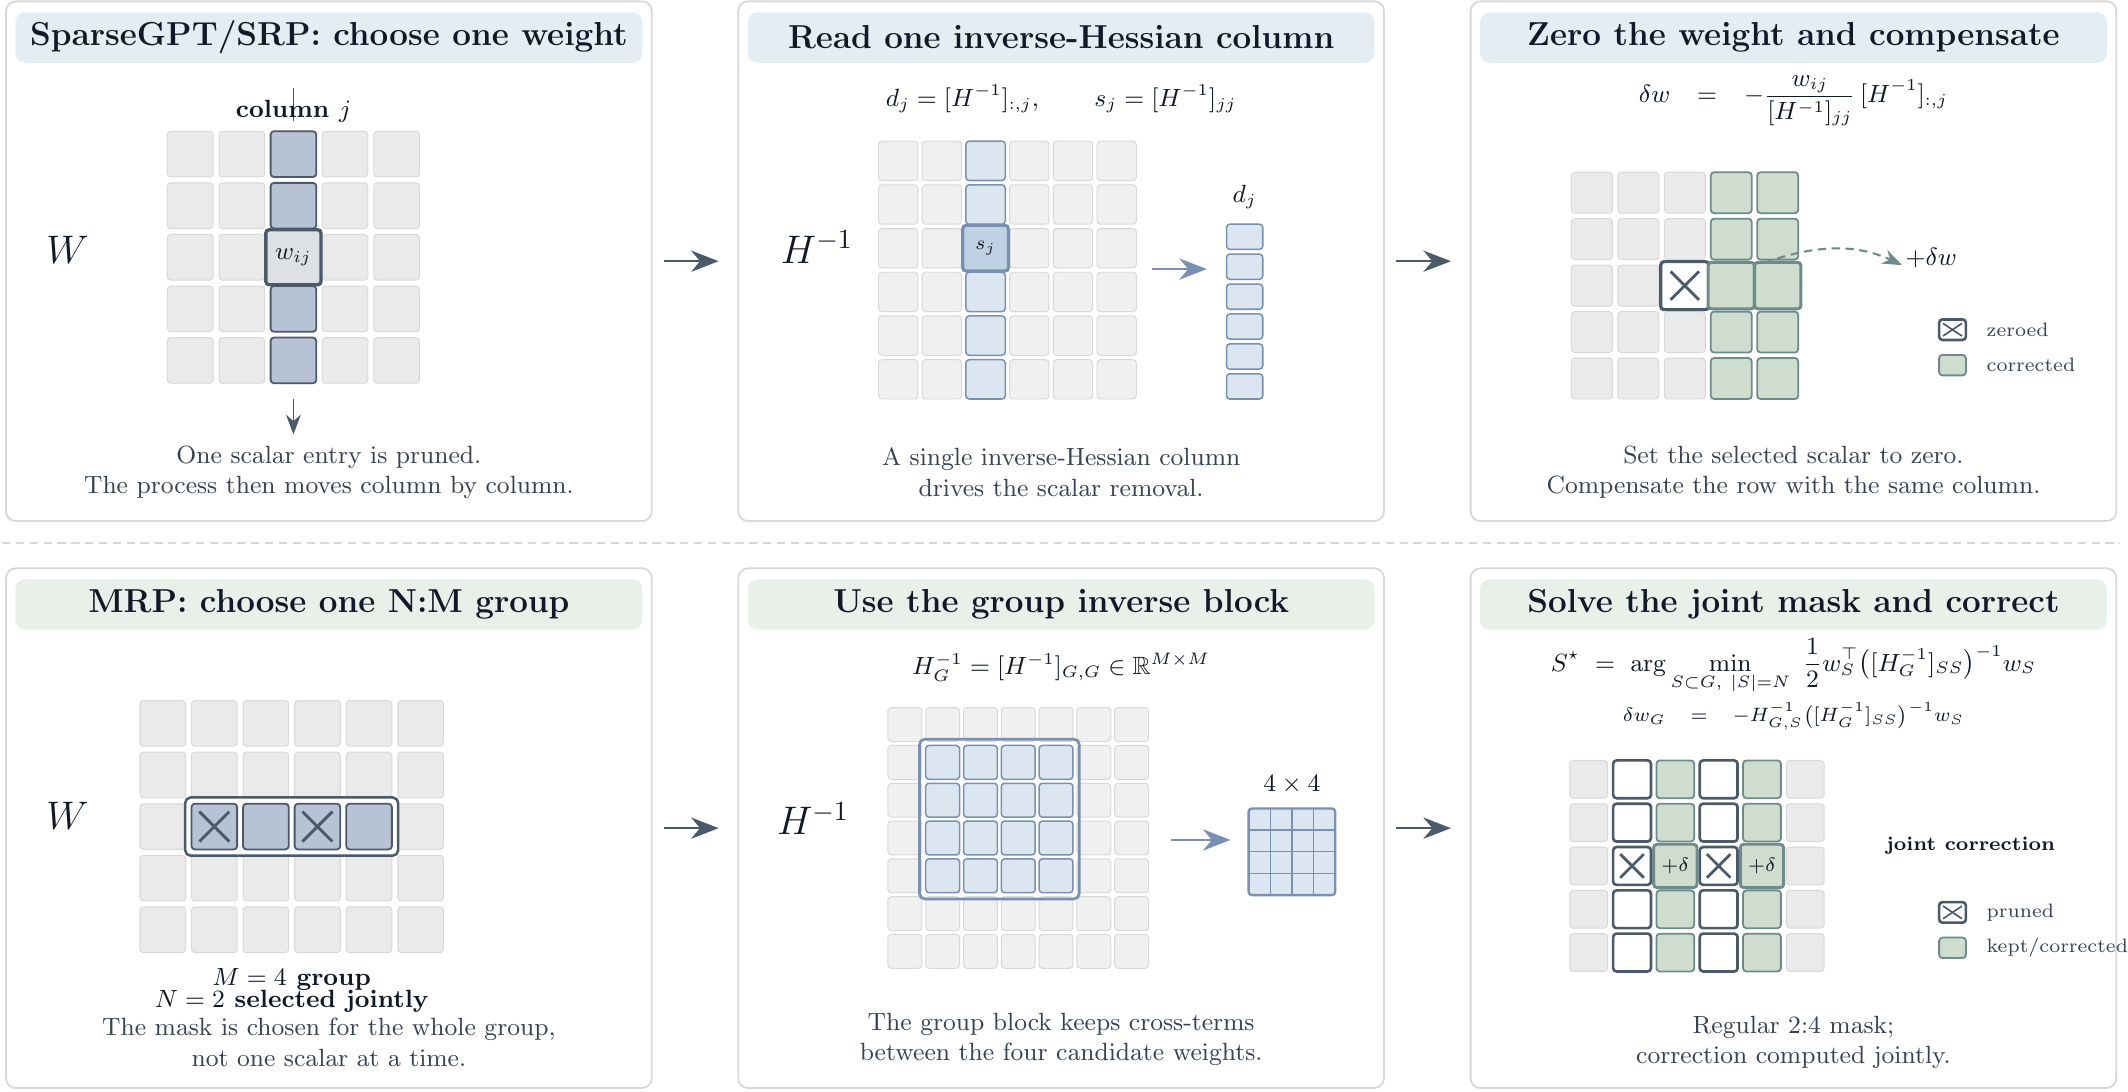
\includegraphics[width=\linewidth]{figures/compression/sparsegpt_mrp_compensation.png}
\caption{Second-order compensation strategies for unstructured and semi-structured pruning.
\emph{(a) SRP (SparseGPT):} one scalar weight is pruned per step; a single column of $\hat{H}^{-1}$ supplies the compensation direction.
\emph{(b) MRP:} the entire N:M group is pruned jointly; the block $(\hat{H}^{-1}_{MM})^{-1}$ captures interactions among simultaneously removed weights.}
\label{fig:hessian_compensation}
\end{figure}

The two methods above operate at scalar-weight or N:M-group granularity. The next method shifts the removable unit to full Transformer structures — attention heads and FFN filters — and incorporates explicit hardware cost into the mask search.

\subsubsection{Fisher-Based Post-Training Structured Pruning}

The post-training framework of Kwon et al. \cite{kwon2022fast} applies second-order structured pruning without end-to-end post-pruning weight optimization. To find the best binary mask over attention heads and FFN filters subject to a hardware budget, the method frames pruning as a constrained combinatorial optimization problem:
\begin{equation}
	\arg\min_{\mathbf{m}} \mathcal{L}(\mathbf{m})
	\quad \text{s.t.} \quad
	\mathrm{Cost}(\mathbf{m}) \leq C,
\end{equation}
where $\mathrm{Cost}$ is either a FLOPs or measured latency budget. Expanding around the dense mask and applying a diagonal Fisher approximation reduces the search to selecting units with the smallest diagonal Fisher scores subject to the cost constraint. For latency-constrained pruning, a piecewise-linear lookup table replaces the analytical cost model to incorporate real device behavior. Specifically, the per-layer latency is modelled as:
\begin{equation}
	\mathrm{LAT}(\mathbf{m}_{\ell}) =
	\begin{cases}
		0, & \|\mathbf{m}_{\ell}\|_0 = 0, \\
		c, & 0 < \|\mathbf{m}_{\ell}\|_0 \leq T, \\
		a(\|\mathbf{m}_{\ell}\|_0 - T) + c, & \|\mathbf{m}_{\ell}\|_0 > T.
	\end{cases}
\end{equation}
Here, the constant term $c$ captures the fixed overhead of activating a layer at all, while the linear term models the additional cost of each surviving unit beyond threshold $T$. This approximation is what lets the framework incorporate actual device behavior while keeping the search tractable.

\methoddetail{Algorithm Overview}
The method proceeds in four steps: (1) diagonal Fisher scores are computed for head and FFN-filter masks on a small calibration set (2K training examples); (2) a FLOPs- or latency-constrained mask search is solved under the diagonal Fisher objective; (3) a block-diagonal Fisher refinement is applied layer by layer to recover interactions ignored by the diagonal approximation; (4) surviving mask values are tuned by layer-wise linear least-squares reconstruction. Because only mask values are updated, the method avoids end-to-end weight retraining. The paper reports pruning times of 39 seconds on GLUE and 135 seconds on SQuAD, compared to 33 hours for CoFi on MNLI.

Whereas the Fisher framework treats device cost through a simple FLOPs or lookup-table model, the final second-order method described here makes hardware latency a first-class optimization objective and derives per-structure removal scores directly from calibration-based curvature.

\subsubsection{Inference-Aware Structured Second-Order Pruning (ZipLM)}

ZipLM \cite{kurtic2023ziplm} applies an OBS-style reconstruction objective to executable Transformer structures rather than scalar weights. To decide which structure to remove next, ZipLM scores each candidate by the total reconstruction error it would introduce across all output rows, weighted by the local curvature. For a candidate structure $S$ with column mask $\mathbf{M}_S$, this structured saliency score is:
\begin{equation}
	\arg\min_S
	\sum_{i=0}^{d_{\text{row}}}
	\mathbf{W}_{i,\mathbf{M}_S}
	\left(\left(\mathbf{H}^{-1}\right)_{\mathbf{M}_S,\mathbf{M}_S}\right)^{-1}
	\mathbf{W}_{i,\mathbf{M}_S}^{T}.
\end{equation}
After removing a structure, the exact compensation and Hessian update are applied through block Gaussian elimination, so that all subsequent saliency scores remain consistent with the already-pruned state.

\methoddetail{Inference-Aware Search}
ZipLM adds a device-level objective on top of the local second-order scoring. It benchmarks attention and FFN configurations on the target hardware and stores measured runtimes in a lookup table. The global search then minimizes layer-wise structural sensitivity subject to a real speed constraint $\sum_\ell \tau_{\ell,s_\ell} \leq T_{\text{target}}$.

\methoddetail{Algorithm Overview}
ZipLM operates in two phases (see Figure~\ref{fig:ziplm_pipeline}). In the global phase, attention-head and FFN configurations are benchmarked on the target environment and a layer-wise sparsity profile satisfying the speedup requirement is selected. In the local phase, each selected layer is compressed by iteratively scoring candidate structures with the structured saliency metric, applying the optimal weight compensation, and updating the inverse Hessian by block Gaussian elimination. Recovery follows a gradual prune-and-fine-tune schedule with combined task, logit, and token-level distillation losses, at a cost of 8--10 fine-tuning epochs per pruning step.

\begin{figure}[H]
	\centering
	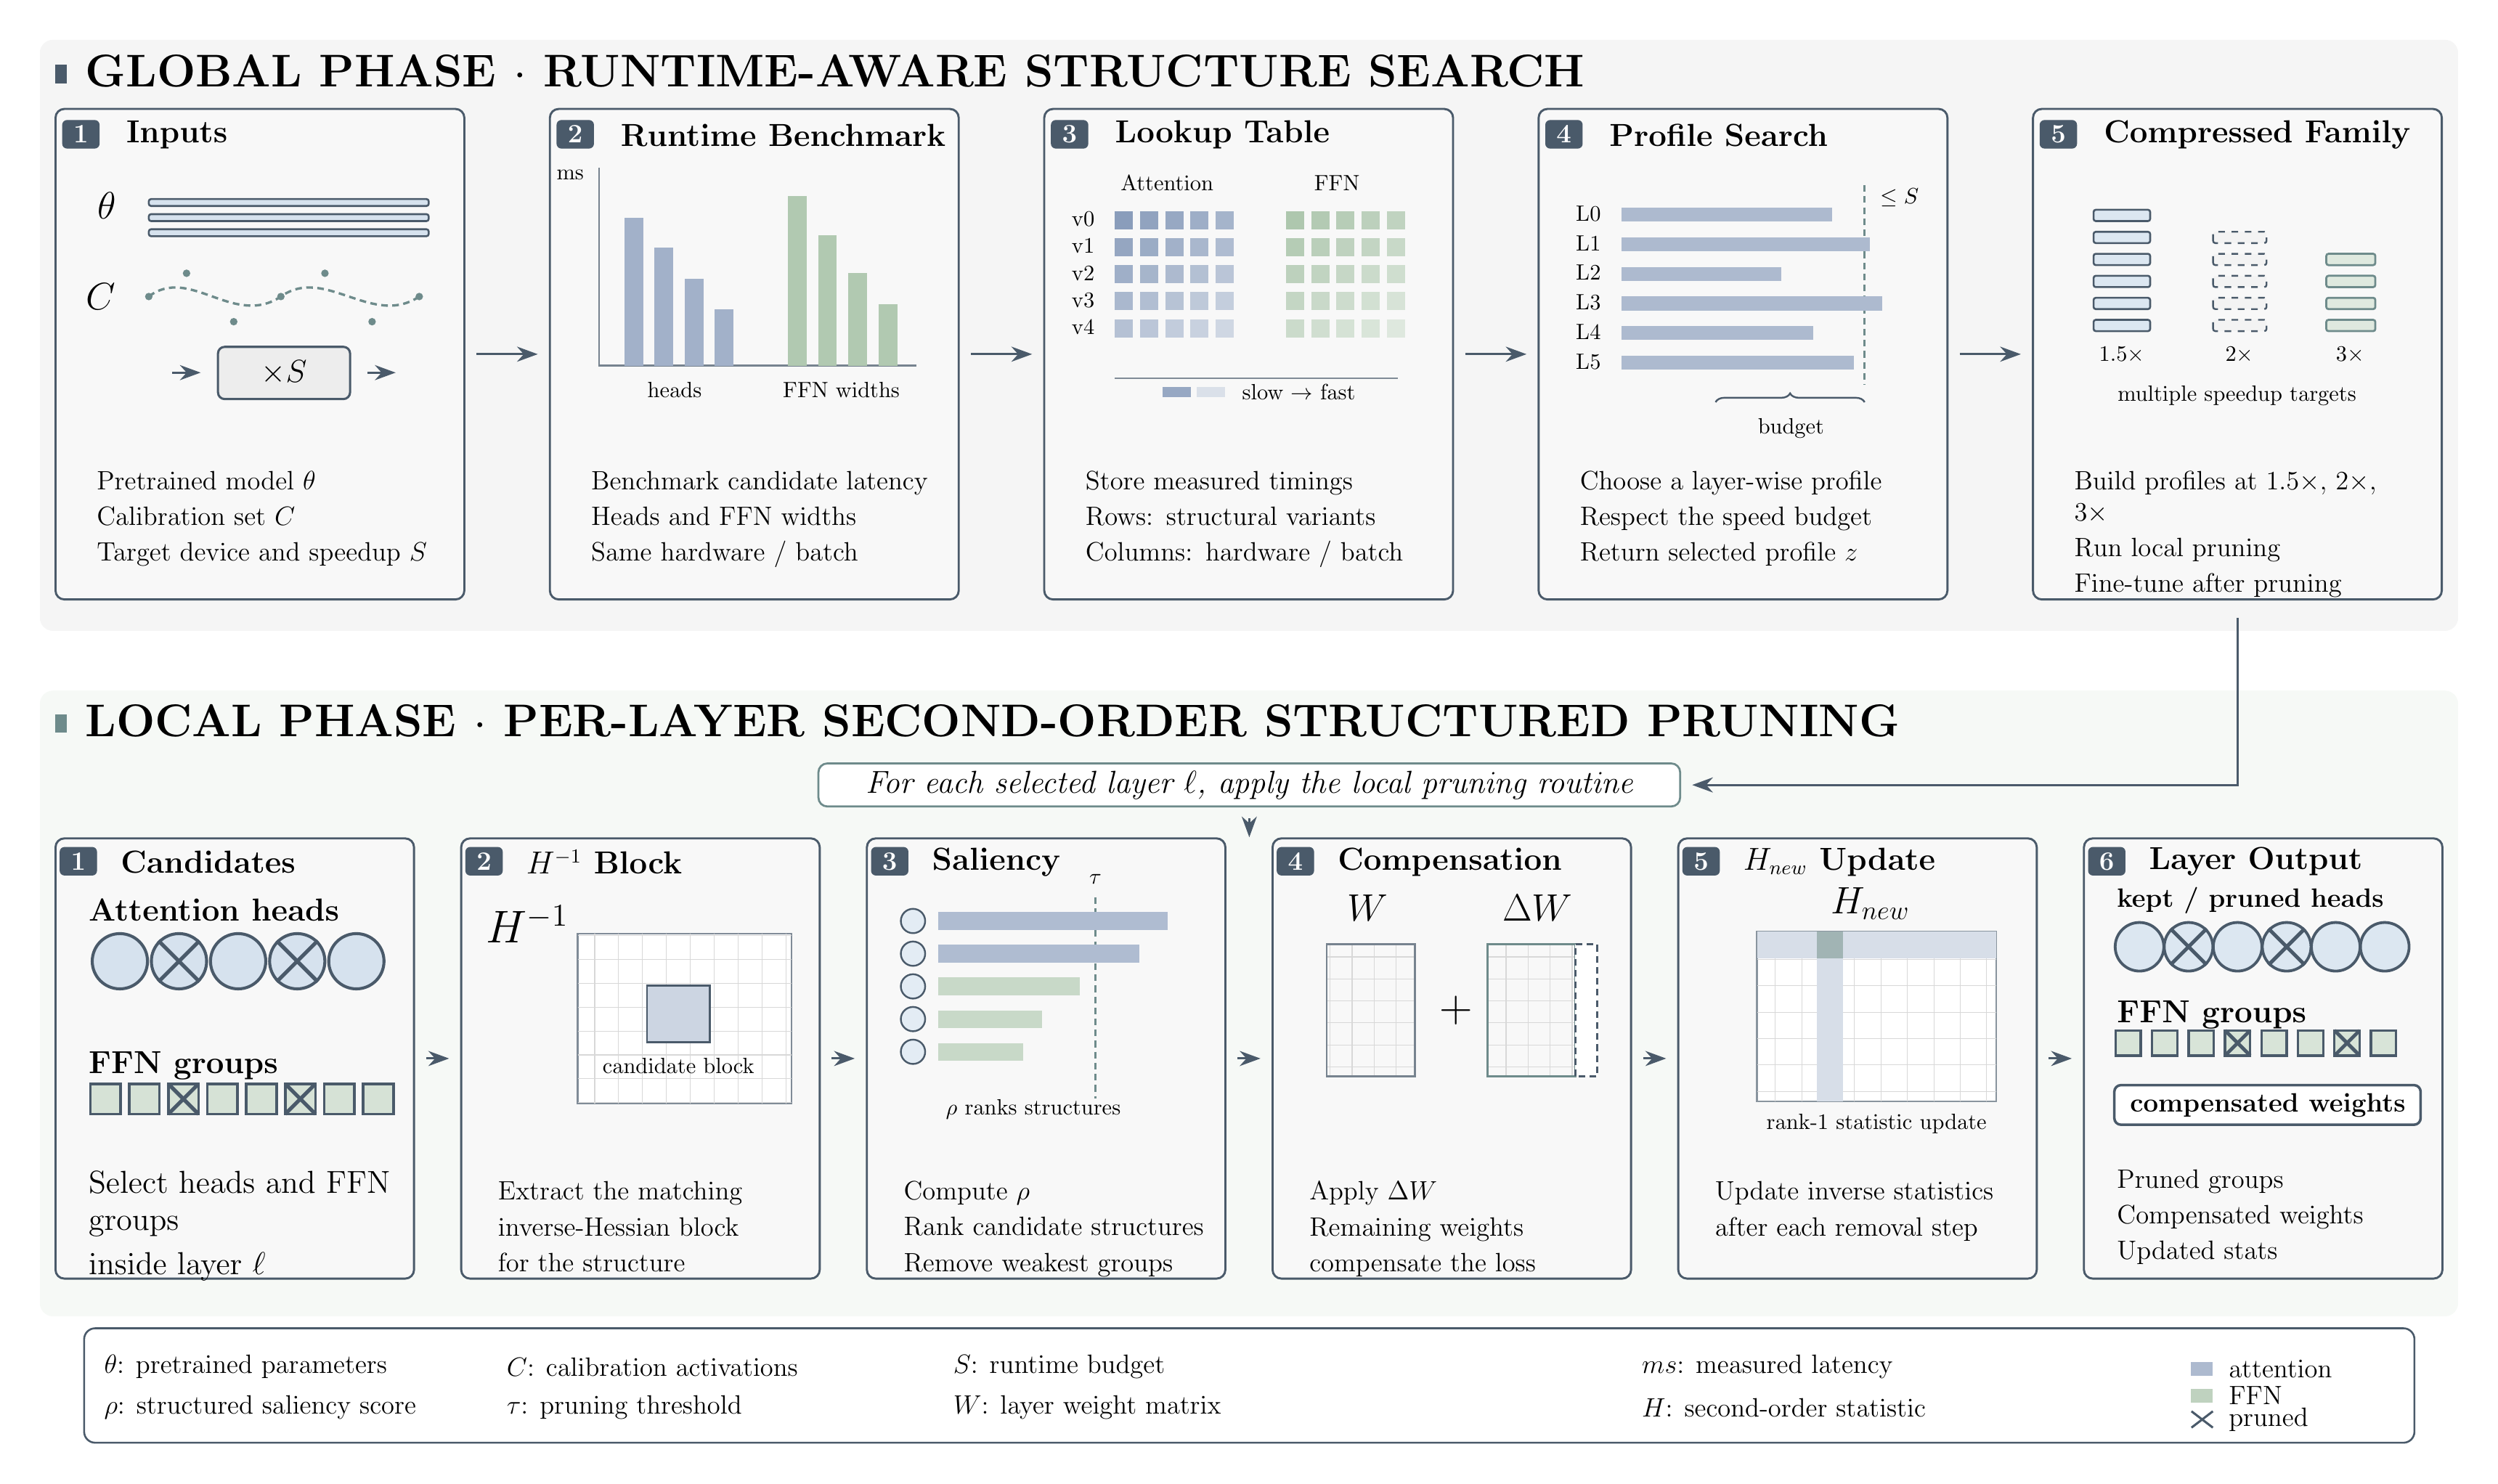
\includegraphics[width=0.96\textwidth]{figures/compression/ziplm_diagram.png}
	\caption{ZipLM pipeline. The global phase benchmarks attention-head and FFN configurations and searches for layer-wise sparsity profiles satisfying the required speedup. The local phase applies second-order structured pruning through inverse-Hessian scoring, compensation updates, and iterative Hessian refinement.}
	\label{fig:ziplm_pipeline}
\end{figure}

The methods covered so far all assign importance scores or solve reconstruction problems in a fixed one-shot or layer-wise fashion. The following section examines a complementary family that treats compression as a search problem over configuration spaces, using cheap proxy signals or population-based evolution to navigate the combinatorial landscape.

\subsection{Proxy- and Search-Based Methods}

Evolutionary and proxy-guided methods search over sparsity configurations or subnetworks using inexpensive proxies or constrained population updates, rather than optimizing explicit masks directly. This section covers three distinct approaches: zero-cost proxies that estimate sub-network quality in a single pass, supernet-based methods that learn masks or sub-networks inside a shared over-parameterized model, and constrained evolutionary frameworks that search over discrete layer-wise compression profiles.

\subsubsection{Zero-Cost Proxies (ZCPs) as Fitness Engines}

Zero-Cost Proxies estimate sub-network quality without full retraining \cite{abdelfattah2021zero,li2023zeroshot}. Each proxy captures a different aspect of network quality through a single forward or backward pass. SynFlow \cite{tanaka2020pruning} measures the total signal flow through a parameter by computing the product of the weight value and its gradient with respect to an all-ones output, which serves as a proxy for how much of the network's capacity passes through that parameter:
\begin{equation}
	I_{i,j} = \frac{\partial (\theta(\mathbf{W}))_{i,j}}{\partial \mathbf{W}_{i,j}} \cdot (\theta(\mathbf{W}))_{i,j}.
\end{equation}
Zen-Score \cite{lin2021zen} takes a different angle and measures expressivity through the sensitivity of the network output to small input perturbations. The final score combines a finite-difference Jacobian norm with a batch-normalization correction term to account for feature-scale differences:
\begin{equation}
	\operatorname{Zen}(f) = \log( \Delta_\alpha(f) ) + \sum_{i\in\mathrm{BN}} \log(\bar{\sigma}_i),
\end{equation}
where $\Delta_\alpha(f; x,\varepsilon) = \|f_\theta(x) - f_\theta(x+\alpha \varepsilon)\|_F / \alpha$ is a finite-difference expressivity estimator. AZ-NAS \cite{lee2024aznasassemblingzerocostproxies} assembles multiple proxy families into a single ranking function, while T-Razor \cite{zhou2022trazor} specializes proxy scoring to Transformers with a diversity-and-saliency aggregate. ZCP evaluation is bounded by one forward or forward-backward pass per candidate, making proxies attractive as inner-loop fitness functions. The trade-off is fidelity: they are fast, but only approximate post-pruning quality. The following section examines methods that go a step further by embedding the pruning search inside a shared model that is itself trained, enabling richer scoring signals at the cost of a more involved optimization procedure.

\subsubsection{Supernet Architecture and Mask Adaptation}

Two complementary approaches are described here. Movement pruning treats the mask scores as learnable parameters updated by gradient descent during fine-tuning, while supernet-based frameworks embed the pruning search inside a shared over-parameterized model that is jointly trained with all sub-networks.

\paragraph{Movement Pruning.}
Movement pruning \cite{sanh2020movement} turns pruning into a learnable masking problem. Each weight $W_{i,j}$ is associated with a trainable score $s_{i,j}$, and the effective parameter is $\widetilde{W}_{i,j} = W_{i,j} \cdot m(s_{i,j})$ where $m$ is a hard or soft threshold. Scores are updated by gradient descent through the mask, replacing one-shot scoring with iterative optimization during fine-tuning.

\paragraph{Supernet-Based Frameworks.}
Supernet methods treat pruning as sub-network selection inside a shared over-parameterized model \cite{Sukthanker2024}. The sandwich rule updates both the full super-network and sampled subnetworks simultaneously; in-place knowledge distillation constrains subnetworks to follow the super-network's output distribution. Structural importance scores are computed directly inside the supernet and used to rank removable units. The additional cost relative to heuristic pruning buys a richer search space and makes structured Pareto optimization feasible.

Both ZCPs and supernet methods ultimately evaluate candidates independently. The following methods instead maintain a population of candidates and use evolutionary operators to navigate the search space, exploiting budget-preserving mutations to focus the search on promising compression profiles.

\subsubsection{Constrained Evolutionary Frameworks}

Two evolutionary methods are examined here: EvoPress, which searches over discrete layer-wise compression profiles under a budget-preserving mutation operator, and DarwinLM, which extends evolutionary search to structured pruning by combining a front-loaded sparsity-level database with training-aware offspring selection.

\paragraph{EvoPress.}
EvoPress \cite{evopress2024} searches over discrete layer-wise compression profiles instead of assigning a single saliency score per layer. A candidate is a configuration $\mathbf{C} = \{c_1,\dots,c_L\}$ where $c_\ell \in \mathcal{S}_\ell$ is the compression level for layer $\ell$. Budget is preserved by level-switch mutation: one layer becomes more compressed only if another becomes less compressed, keeping the global average sparsity $S_{\text{glob}}$ fixed. Mutations are deliberately local, with most offspring differing from the parent by only one or two switches.

Selection proceeds in multiple rounds with increasing token budgets and decreasing survivor counts. This progressive tournament ensures that accurate but expensive fitness evaluations are reserved for the most promising candidates. Formally, the population update at round $r$ is:
\begin{equation}
	\mathcal{P}^{(r+1)} =
	\operatorname{Top}_{n_{r+1}}
	\left(
	\left\{
	\mathcal{F}_{T_r}(C) \mid C \in \mathcal{P}^{(r)}
	\right\}
	\right),
	\qquad
	T_1<T_2<\cdots,\;
	n_1>n_2>\cdots,
\end{equation}
where the fitness signal $\mathcal{F}_{T_r}(C)$ is the negative KL divergence to the reference model evaluated over $T_r$ tokens. This progressive evaluation scheme is what makes EvoPress practically efficient: early rounds use few tokens to discard poor candidates quickly, reserving the full calibration budget for finalists. The method converges in approximately 5--6 GPU hours for a standard Llama-2-7B sparsity search.

\begin{figure}[H]
\centering
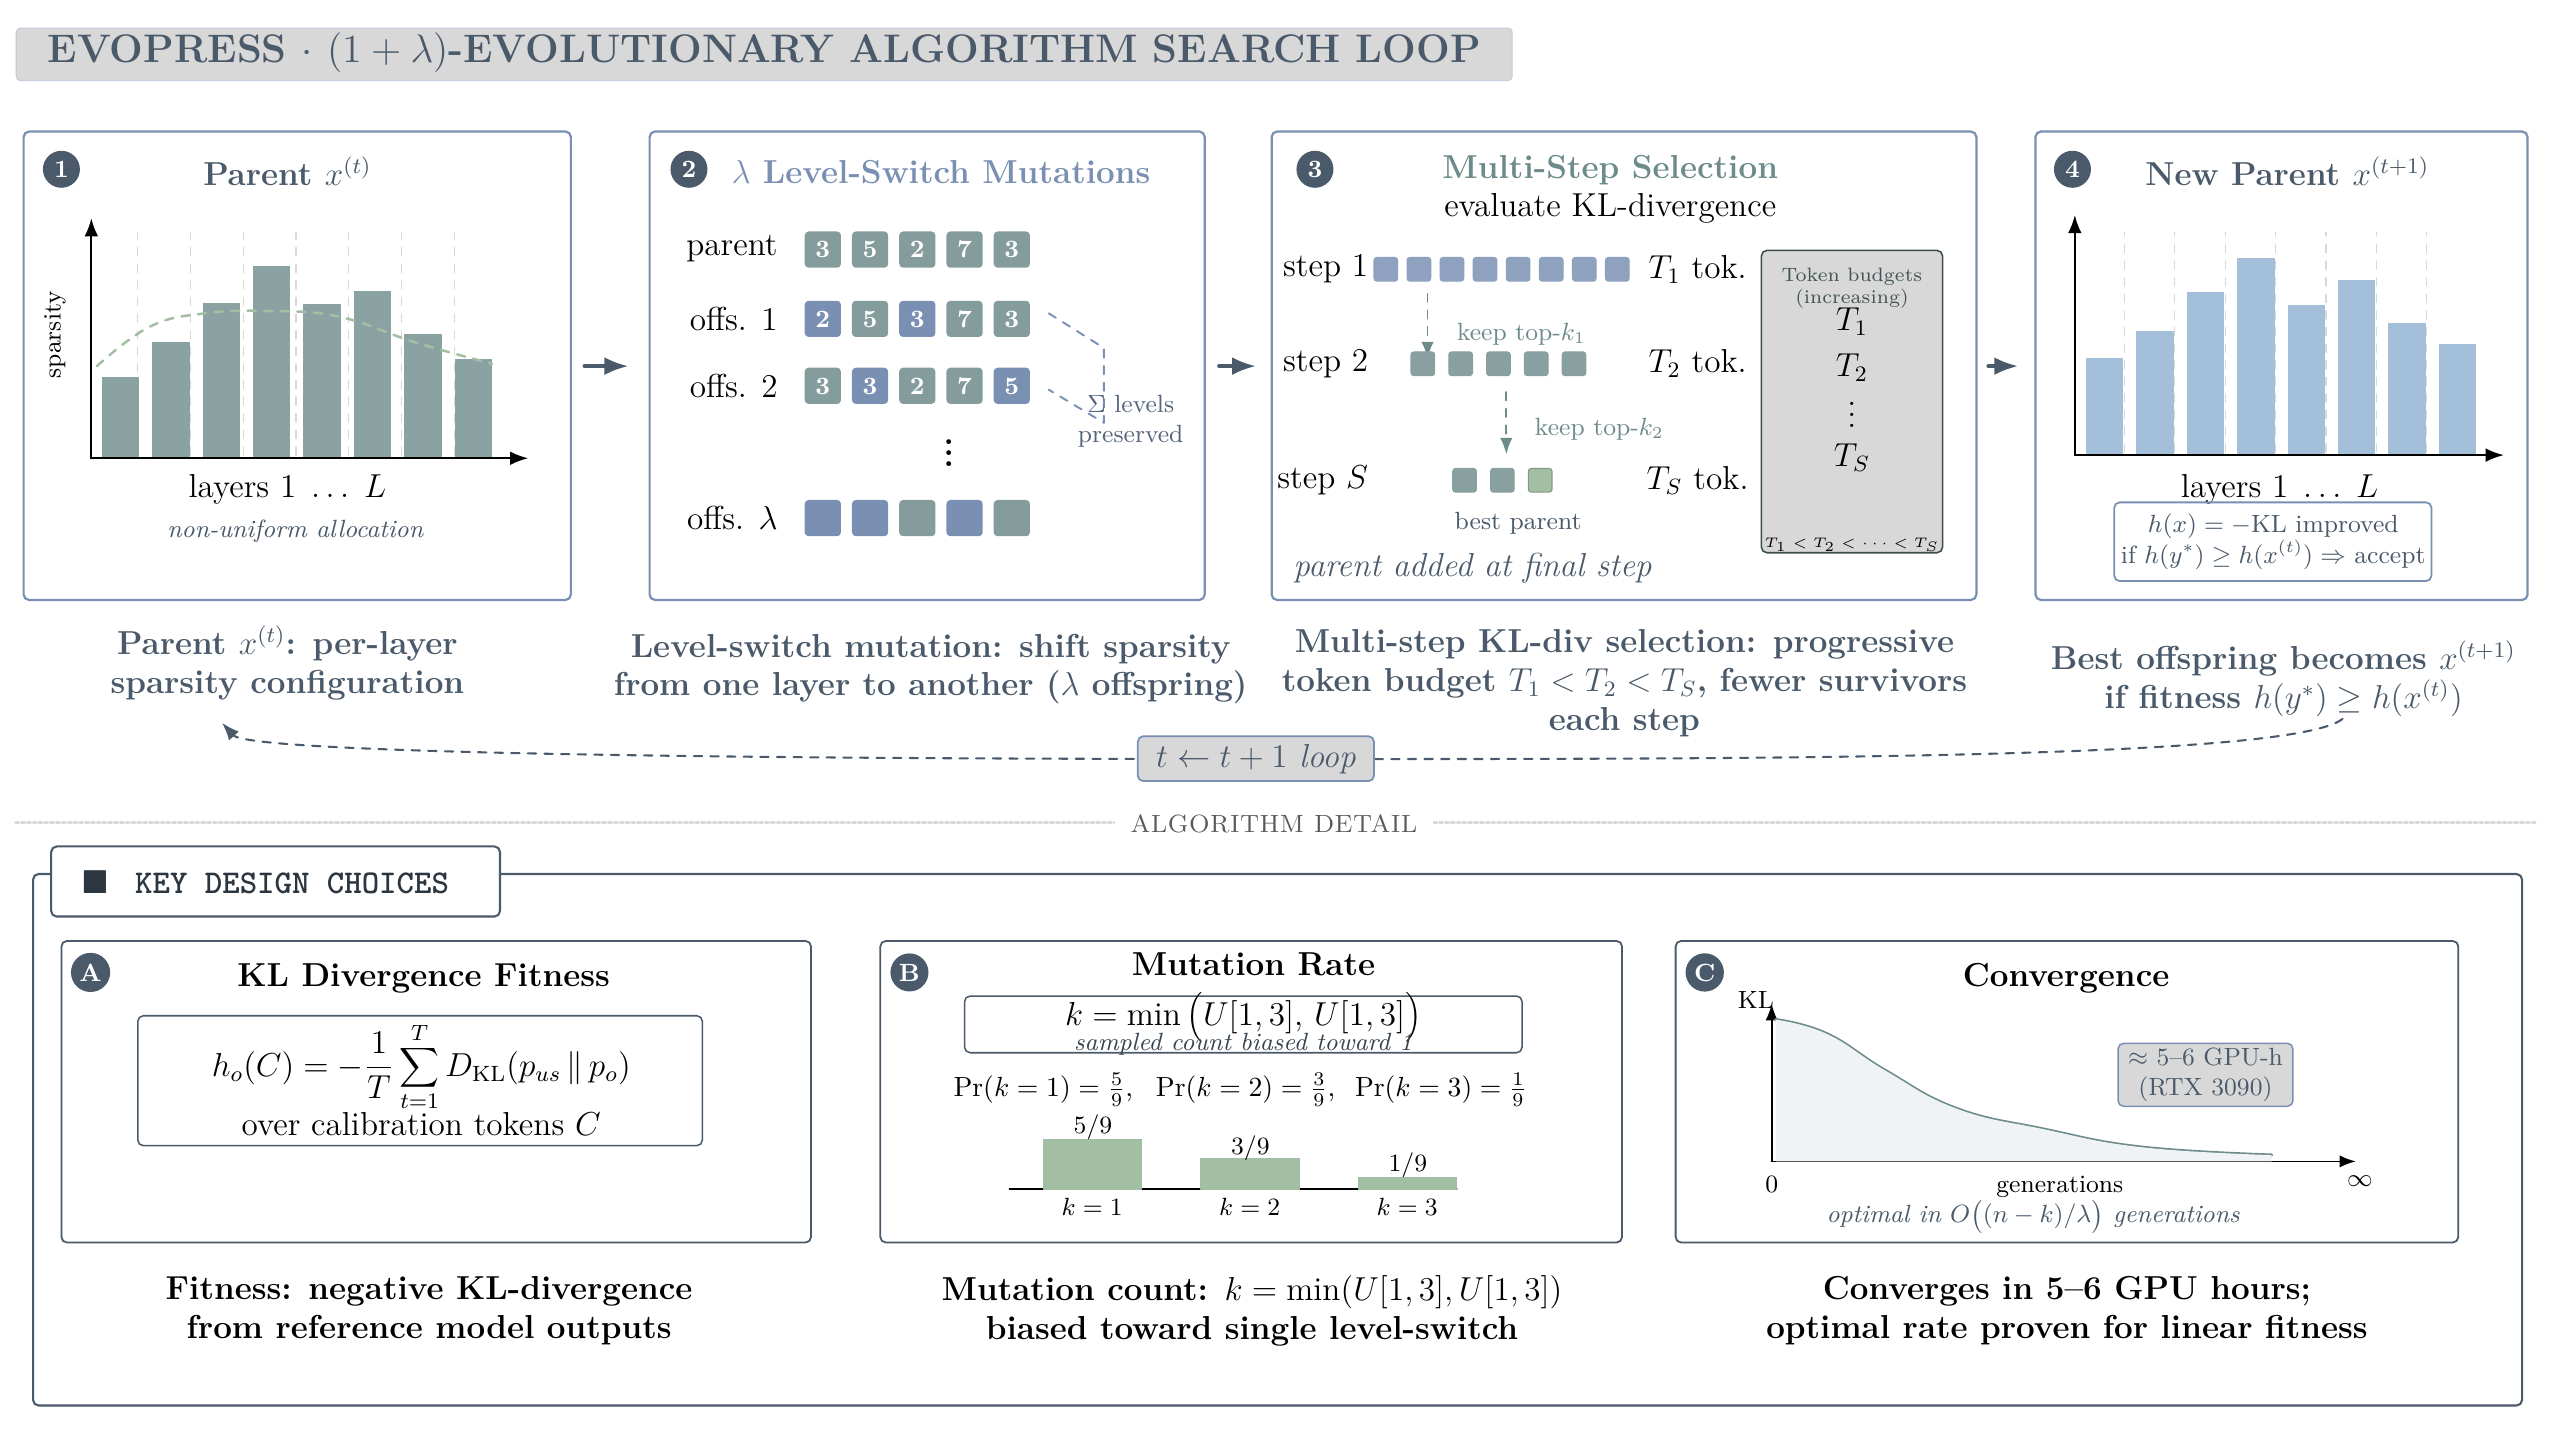
\includegraphics[width=0.94\linewidth,height=0.50\textheight,keepaspectratio]{figures/compression/evopress_search_loop.png}
\caption{EvoPress $(1+\lambda)$ evolutionary search loop for dynamic LLM compression \citep{evopress2024}. The method applies budget-preserving level-switch mutation and progressively evaluates candidates with larger calibration budgets.}
\label{fig:evolutionary_pruning_flow}
\end{figure}
\FloatBarrier

\paragraph{DarwinLM.}
DarwinLM \cite{darwinlm2025} extends evolutionary search to \emph{structured} pruning by unifying OBS-style second-order pruning with a training-aware offspring selection strategy. It differs from EvoPress on three axes: structured granularity (heads and FFN channels), front-loaded Hessian computation stored in a sparsity-level database (SLD), and fitness measured after a short lightweight finetune rather than from the one-shot pruned model.

\methoddetail{Sparsity Level Database}
For each module, DarwinLM solves the structured OBS problem at $N_l$ equally-spaced sparsity levels and stores the pruned-and-compensated weights. Concretely, for a given column mask $M$ specifying which columns to prune, the optimal mask minimizes the reconstruction error across all output rows, and the optimal compensation adjusts the surviving weights to absorb the error introduced by the pruned ones:
\begin{align}
	M^* &= \arg\min_{M}\sum_{i=1}^{d_{\mathrm{row}}}
		\mathbf{W}_{i,M}\bigl(\hat{H}^{-1}_{MM}\bigr)^{-1}\mathbf{W}_{i,M}^\top, \\
	\delta^* &= -\mathbf{W}_{:,M}\bigl(\hat{H}^{-1}_{MM}\bigr)^{-1}\hat{H}^{-1}_{M,:}.
\end{align}
During search, candidate models are assembled by looking up stored entries, avoiding any Hessian recomputation.

\methoddetail{Training-Aware Selection}
Each candidate receives a short lightweight finetune before evaluation. The motivation is that one-shot pruned quality is a weak predictor of post-training accuracy; even a brief finetune on 10K--200K tokens provides a signal strongly correlated with full post-training performance. The fitness of candidate $C_k$ is therefore the KL divergence between the dense reference and the briefly fine-tuned candidate:
\begin{equation}
	\mathcal{F}(C_k) = D_{\mathrm{KL}}\!\bigl(\hat{M}\,\|\,\operatorname{finetune}(C_k,\, T_f)\bigr).
\end{equation}
Selection uses three progressive rounds ($T_f \in \{10\text{K}, 50\text{K}, 200\text{K}\}$ tokens) with decreasing survivor counts. The SLD must be computed once per model and sparsity range, making the upfront cost proportional to $L \cdot N_l$ structured OBS operations. DarwinLM compresses Llama-2-7B to 2.7B parameters with higher downstream accuracy than ShearedLlama using $5\times$ fewer post-training tokens (10B vs.\ 50B).

\begin{figure}[H]
\centering
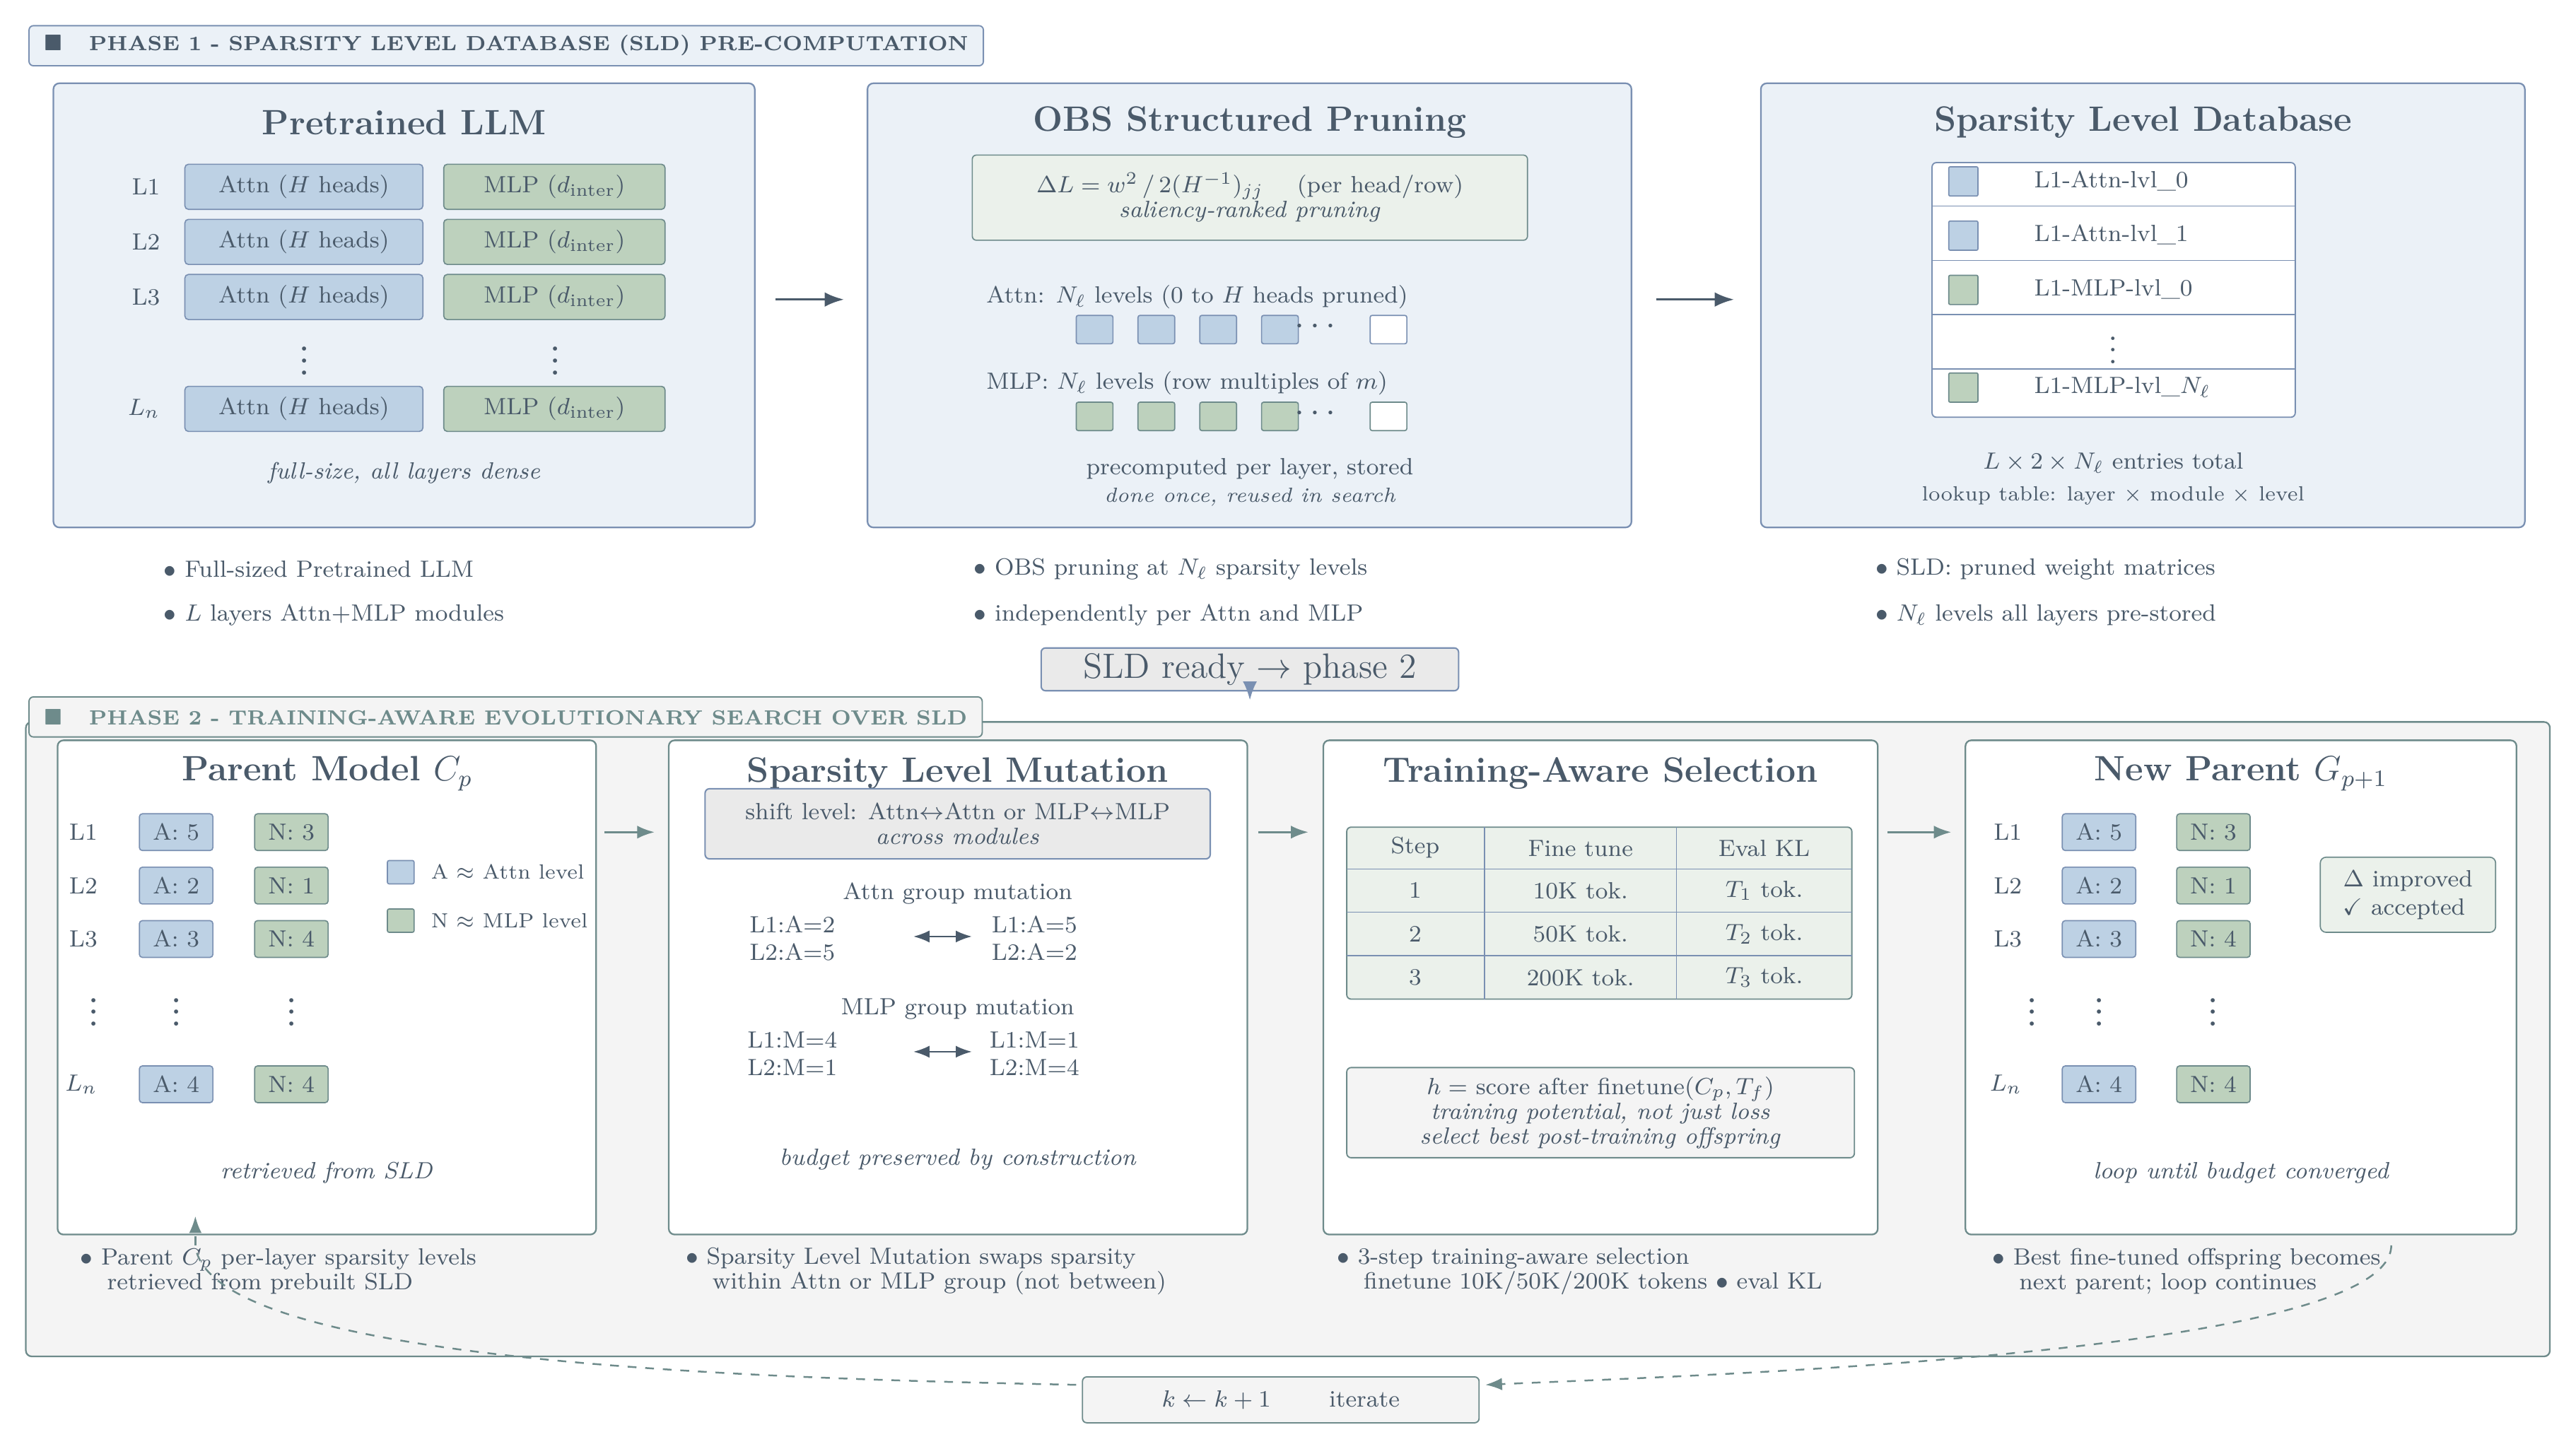
\includegraphics[width=0.94\linewidth,height=0.50\textheight,keepaspectratio]{figures/compression/darwinlm_search_loop.png}
\caption{DarwinLM search loop \citep{darwinlm2025}. The method first builds a sparsity-level database with OBS-style structured pruning, then performs training-aware evolutionary selection over stitched candidate models.}
\label{fig:darwinlm_pruning_flow}
\end{figure}

\begin{table}[H]
	\centering
	\caption{Computational overhead profile of representative pruning methods.}
	\label{tab:unstructured_comparison}
	\begin{tabular}{@{}p{2.4cm}p{3.6cm}p{3.8cm}@{}}
		\toprule
		\textbf{Method} & \textbf{Dominant preprocessing cost} & \textbf{Additional requirement} \\ \midrule
		Magnitude \cite{han2015deep} & Linear scan $O(|W|)$ & None \\
		Wanda \cite{sun2023simple} & Activation collection + linear scoring & Small calibration set ($\approx$128 samples) \\
		CoFi \cite{xia2022structured} & Multi-epoch joint mask and weight optimization & Task-specific teacher; $\approx$33 h for MNLI \\
		LLM-Pruner \cite{ma2023llmpruner} & Forward/backward scoring over dependency groups & LoRA recovery ($\approx$2.5 h on RTX 4090) \\
		SparseGPT \cite{frantar2023sparsegpt} & $O(d_{\mathrm{in}}^2 d_{\mathrm{out}} + d_{\mathrm{in}}^3/B)$ per layer & Calibration Hessian \\
		MRP \cite{zhao2024pruning} & Group-wise exact or approximate mask search & Block curvature updates per N:M group \\
		Fast PTPF \cite{kwon2022fast} & Diagonal / block Fisher estimation + mask tuning & Calibration set; optional latency lookup table \\
		ZipLM \cite{kurtic2023ziplm} & Layer-wise Hessian updates + runtime-table search & Calibration set + hardware benchmarking pass \\
		Movement \cite{sanh2020movement} & Iterative fine-tuning with mask parameter updates & Full training data \\
		EvoPress / DarwinLM \cite{evopress2024,darwinlm2025} & Population search over compression profiles & 1--6 GPU-hours; SLD pre-computation for DarwinLM \\ \bottomrule
	\end{tabular}
\end{table}

Having described all methods and their preprocessing costs, we now turn to their empirical performance. The results below are organized by pruning regime, since methods operating at different granularities or targeting different hardware objectives are not directly comparable on a single axis.

\subsection{Empirical Comparison}

All perplexity values, accuracy scores, and performance results are consolidated in the following subsections. Methods are organized by pruning regime — unstructured and semi-structured, structured, and evolutionary — because direct comparison across regimes would conflate different hardware targets, recovery budgets, and evaluation protocols. Readers should therefore interpret each sub-table on its own terms before drawing cross-regime conclusions.

\subsubsection{Unstructured and Semi-Structured (N:M) Results}

Table~\ref{tab:unsupported_comparison} summarizes the perplexity trade-off at 50\% unstructured sparsity and at the 2:4 semi-structured operating point. Wanda and SparseGPT substantially outperform magnitude pruning, with their gap widening at smaller model sizes. At the 2:4 operating point, SparseGPT's perplexity penalty reduces with model scale, reaching under 0.4 points for OPT-175B.

\begin{table}[H]
	\centering
	\caption{Unstructured (50\%) and Semi-Structured (2:4) Pruning on WikiText Perplexity. Wanda results are on LLaMA models; SparseGPT results are on OPT models.}
	\label{tab:unsupported_comparison}
	\begin{tabular}{@{}llcccc@{}}
		\toprule
		\textbf{Model} & \textbf{Setting} & \textbf{Dense PPL} & \textbf{Magnitude PPL} & \textbf{SparseGPT PPL} & \textbf{Wanda PPL} \\
		\midrule
		LLaMA-7B  & 50\% unstr. & 5.68 & 17.29 & 7.22 & 7.26 \\
		LLaMA-13B & 50\% unstr. & 5.09 & 20.21 & 6.21 & 6.15 \\
		LLaMA-30B & 50\% unstr. & 4.77 & 7.54  & 5.31 & 5.24 \\
		LLaMA-65B & 50\% unstr. & 3.56 & 5.90  & 4.57 & 4.57 \\
		\midrule
		OPT-13B   & 50\% unstr. & 10.13 & 1.2e4 & 11.17 & -- \\
		OPT-30B   & 50\% unstr. & 9.56  & 168   & 9.79  & -- \\
		OPT-66B   & 50\% unstr. & 9.34  & 4.2e3 & 9.32  & -- \\
		OPT-175B  & 50\% unstr. & 8.35  & 4.3e4 & 8.21  & -- \\
		\midrule
		OPT-13B   & 2:4 semi    & 10.13 & --    & 12.96 & -- \\
		OPT-30B   & 2:4 semi    & 9.56  & --    & 10.90 & -- \\
		OPT-66B   & 2:4 semi    & 9.34  & --    & 10.09 & -- \\
		OPT-175B  & 2:4 semi    & 8.35  & --    & 8.74  & -- \\
		\bottomrule
	\end{tabular}
\end{table}

The unstructured and semi-structured results above are reported on language modelling perplexity, which is the natural metric when no end-to-end fine-tuning follows pruning. The structured methods below optimize for a different objective — task accuracy at a target speedup or compression ratio — and are therefore evaluated on downstream benchmarks.

\subsubsection{Structured Pruning Results}

Table~\ref{tab:structured_summary} consolidates headline results across the structured methods. CoFi and ZipLM address encoder models with explicit speedup targets; LLM-Pruner addresses decoder LLMs with accuracy retention under structural compression; the post-training Fisher framework emphasizes cost-constrained pruning with near-zero recovery overhead.

\begin{table}[H]
	\centering
	\caption{Structured Pruning: Headline Results Across Methods and Settings}
	\label{tab:structured_summary}
	\begin{tabular}{@{}llp{4.5cm}p{4.5cm}@{}}
		\toprule
		\textbf{Method} & \textbf{Model} & \textbf{Setting} & \textbf{Key Result} \\
		\midrule
		LLM-Pruner \cite{ma2023llmpruner}
		  & LLaMA-7B & 20\% prune ratio, zero-shot avg. & 98.6\% accuracy retention after LoRA recovery \\
		  & LLaMA-7B & 50\% prune ratio & 83.6\% accuracy retention after LoRA recovery \\
		  & Vicuna-7B & 20\% prune ratio & 96.1\% accuracy retention after LoRA recovery \\
		\midrule
		CoFi \cite{xia2022structured}
		  & BERT Base & $\approx$12$\times$ speedup (MNLI) & 80.6 acc. vs. 78.8 for TinyBERT$_4$ at same speedup \\
		  & BERT Base & $\approx$12$\times$ speedup (SST-2) & 90.6 acc. vs. 89.7 for TinyBERT$_4$ \\
		  & BERT Base & $\approx$8.7$\times$ speedup (SQuAD) & 82.6 F1, matching TinyBERT$_4$ at same speedup \\
		\midrule
		Fast PTPF \cite{kwon2022fast}
		  & BERT Base & FLOPs-constrained & 60--70\% FLOPs with $\leq$1\% accuracy drop on GLUE/SQuAD \\
		  & BERT Base & Latency, batch 32 & $1.34\times$ geometric-mean speedup, NVIDIA V100 \\
		  & BERT Base & Latency, batch 256 & $1.47\times$ geometric-mean speedup, NVIDIA V100 \\
		  & BERT Base & End-to-end time & 39 s on GLUE, 135 s on SQuAD (vs. 33 h for CoFi) \\
		\midrule
		ZipLM \cite{kurtic2023ziplm}
		  & BERT Base & $2\times$ speedup (QNLI/MNLI) & 91.4 / 84.8 acc. (dense: 91.5 / 84.8), 38M params \\
		  & BERT Base & $5\times$ speedup (QNLI/MNLI) & 90.8 / 84.0 acc., 12--13M params \\
		  & BERT Base & $10\times$ speedup (QNLI/MNLI) & 88.6 / 82.7 acc., $\approx$5M params \\
		  & BERT Large & $5\times$ speedup (SQuAD) & 90.8 F1, 48.5M params \\
		  & BERT Large & $10\times$ speedup (SQuAD) & 89.1 F1, 20.9M params \\
		\bottomrule
	\end{tabular}
\end{table}

The structured results above cover encoder models evaluated on NLU and reading-comprehension benchmarks. The evolutionary methods below operate on decoder LLMs at much larger scale and report perplexity alongside zero-shot task averages, reflecting the different model families and evaluation conventions in that line of work.

\subsubsection{Evolutionary and Search-Based Results}

EvoPress and DarwinLM are evaluated on both depth pruning and unstructured sparsity. Table~\ref{tab:search_summary} highlights the main findings. For depth pruning, EvoPress substantially outperforms heuristic methods (ShortGPT, Cosine Similarity, Shortened Llama) at all sparsity levels, with the gap widening considerably at 25\%+ sparsity where heuristic methods catastrophically degrade. For unstructured sparsity, EvoPress consistently improves on both uniform allocation and OWL across models and sparsity levels, with the largest gains at 70\% sparsity on more sensitive architectures such as Llama-3-8B (WikiText PPL: 28.76 vs. 48.07 for OWL).

\begin{table}[H]
	\centering
	\caption{Evolutionary Methods: Selected Results on Mistral-7B-v0.3 and Llama-2-7B. EvoPress depth-pruning versus ShortGPT and Shortened Llama; EvoPress unstructured sparsity versus Uniform and OWL.}
	\label{tab:search_summary}
	\begin{tabular}{@{}llllccc@{}}
		\toprule
		\textbf{Setting} & \textbf{Model} & \textbf{Sparsity} & \textbf{Method} & \textbf{Wiki2$\downarrow$} & \textbf{C4$\downarrow$} & \textbf{Task Avg.} \\
		\midrule
		\multirow{6}{*}{Depth pruning}
		  & \multirow{3}{*}{Mistral-7B} & 25\% & EvoPress      & \textbf{8.66}  & \textbf{12.04} & -- \\
		  &                             & 25\% & ShortGPT      & 43.26 & 40.16 & -- \\
		  &                             & 25\% & Shortened LLaMA & 14.94 & 19.30 & -- \\
		  \cmidrule{2-7}
		  & \multirow{3}{*}{Llama-2-7B} & 25\% & EvoPress      & \textbf{9.15}  & \textbf{11.46} & -- \\
		  &                              & 25\% & ShortGPT      & -- & -- & -- \\
		  &                              & 25\% & Shortened LLaMA & -- & -- & -- \\
		\midrule
		\multirow{6}{*}{Unstructured}
		  & \multirow{3}{*}{Mistral-7B} & 70\% & EvoPress  & \textbf{14.42} & \textbf{16.46} & \textbf{53.8} \\
		  &                             & 70\% & OWL       & 17.22 & 21.66 & 51.9 \\
		  &                             & 70\% & Uniform   & 23.08 & 30.03 & 49.9 \\
		  \cmidrule{2-7}
		  & \multirow{3}{*}{Llama-2-7B} & 50\% & EvoPress & \textbf{6.22}  & \textbf{8.52}  & \textbf{63.2} \\
		  &                              & 50\% & OWL      & 6.38  & 8.77  & 62.9 \\
		  &                              & 50\% & Uniform  & 6.40  & 8.87  & 62.4 \\
		\bottomrule
	\end{tabular}
\end{table}

To situate these individual results within the broader literature, Table~\ref{tab:comprehensive_pruning} below gathers representative publications from 2020 to 2025, spanning all pruning granularities and a range of target architectures and benchmarks. It is intended as an orientation map rather than a direct ranking, since publication-specific choices of evaluation protocol, base model, and fine-tuning budget make cell-by-cell comparison misleading.

\subsubsection{Aggregated SOTA Landscape}

Table~\ref{tab:comprehensive_pruning} consolidates the broader pruning landscape across pruning granularity, speedup regime, and retained accuracy.

\begin{table}[H]
	\begin{adjustwidth}{-1.2cm}{0cm}
		\centering
		\caption{Pruning Performance Overview}
		\label{tab:comprehensive_pruning}
		\begin{tabular}{@{}lllp{4.5cm}cccc@{}}
			\toprule
			\textbf{Publication} & \textbf{Year} & \textbf{Method Type} & \textbf{Dataset} & \textbf{Speed-Up} & \textbf{Model Size} & \textbf{Accuracy} \\ \midrule
			PoWER-BERT & 2020 & Token Pruning & GLUE, IMDB, RACE & 2.8$\times$ (E) & $>$100\% & 99\% \\
			Vis Pruning & 2021 & Head/Weight (DeiT) & ImageNet-1K & 1.76$\times$ (T) & 55.5\% & 98.1\% \\
			JMC + DISP & 2021 & Head/Weight + KD & SST-2, SemEval, SNLI & 8$\times$ (E) & 26.6\% & 96.5\% \\
			PTPF & 2022 & Head/Weight (BERT) & GLUE, SQuAD & 1.56$\times$ (E) & 70\% & 99\% \\
			Dropping Layers & 2022 & Layer Pruning (BERT) & GLUE & 1.5$\times$ (E) & 60\% & 96.7\% \\
			Token Pruning & 2022 & Token Pruning (RoBERTa) & GLUE, SQuAD & 1.96$\times$ (E) & $>$100\% & 99\% \\
			Pruning for FT & 2024 & Head + Weight (ViT) & CIFAR100, TinyImageNet & - & $\sim$36\% & 94.8\% \\
			Need for Speed & 2024 & Head + Weight (BERT) & GLUE & 1.67$\times$ (T) & - & 98\% \\
			Zero-TPrune & 2024 & Token Pruning (DeiT) & ImageNet & 1.45$\times$ (E) & $>$100\% & 99.6\% \\
			EvoPress & 2025 & Evolutionary (Mistral-7B) & Wiki2, C4, FW, ArcC & - & 30\% & 96\% \\
			Supernet-NAS & 2024 & NAS (Phi-2/3, Llama) & Winogrande, ARC, MMLU & 1.2$\times$ (E) & $\sim$90\% & $\sim$99\% \\
			\bottomrule
		\end{tabular}
	\end{adjustwidth}
\end{table}